%\subsection{Segmentation de l'environnement intérieur}
%segmentation par l'utilisateur
%\subsection{Création d'une base de connaissance}
%utilisation opencv
%creation du dictionnaire
%calcul du descripteur des objets -> detail sur le nombre d'objet et sur le nombre d'exemplaire
%test sur une base composé de mesh et sur une autre composé de nuage de point
%\subsection{Reconnaissance des objets} 
%simple comparaison avec le descripteur
%TODO voir ce qu'on peut mettre dans cette section

\subsection{Objectif}
%interface
Le but de cette seconde application est de pouvoir modifier un environnement d'une pièce intérieur au travers d'une interface
simple et intuitive. 
Pour cela, nous allons dans un premier temps récupérer un nuage de point d'une pièce intérieur. Puis à partir
de ce nuage de point, nous allons segmenter la pièce afin de pouvoir détecter des objets à l'intérieur de celle-ci.
L'utilisateur doit ensuite sélectionner un objet, ce qui déclenchera l'apparition d'une liste contenant un ensemble de modèle 3D
d'objet équivalant à celui sélectionné. L'utilisateur n'a plus qu'à sélectionner l'objet qui lui convient dans la liste
afin de l'ajouté dans un autre environnement 3D présent dans l'application.\\

Lors de ce scénario, nous pouvons voir qu'il y a deux grandes étapes qu'il faudra réaliser dans l'application. Tout d'abord il faut 
segmenter le nuage de point de la pièce dans le but de détecter des objets. Puis il faut reconnaître les objets détectés afin
d'afficher la bonne liste d'objet 3D. Nous avons décidé, pour faciliter le développement, de laissé l'utilisateur sélectionner
l'objet qu'il souhaite dans le nuage de point afin de ne pas avoir à développer la détection d'objet dans le nuage de point.
Pour cela nous nous inspirons des travaux de T. Shao et al\cite{interactiveSeg} et de J. Xiao et al\cite{interactionSeg2}.
Il nous reste donc à reconnaitre l'objet sélectionner par l'utilisateur.

\subsection{Création de la base d'apprentissage}
Afin de pouvoir reconnaître un objet, nous avons besoin d'un base d'apprentissage contenant les descripteurs d'un ensemble
d'objets. Pour créer cette base, nous utilisons la représentation du \og bag of word \fg ainsi que la méthode d'apprentissage 
automatique SVM\cite{SVM} disponible dans la librairie opencv. Pour la création de notre base nous utilisons une soixantaine
d'image de six objets différents. Les nuages de points dont nous nous sommes servis pour la création de notre base viennent de 
K. Lai et al\cite{Base1} et de M. Firman\cite{generalBase} qui a regroupé un ensemble de base d'objet provenant de caméra 3D.\\

Le descripteur que nous utilisons pour cette application est le descripteur FPFH\cite{FPFH} qui est l'un des plus efficaces dans la
reconnaissance d'objet à partir de nuage de point. Nous calculons ce descripteur sur l'ensemble des images de notre base afin de
créer le dictionnaire de notre bag of word. A cette étape du développement nous avons créé le dictionnaire, il faut alors recalculer
le descripteur sur chacun des objets afin de déterminer les caractèristiques de chaque objet. Cela nous permet d'obtenir un histogramme
pour chaque objet comportant les caractèristique qu'il contient et le nombre de fois qu'il apparaît. Il ne reste plus qu'à utiliser
le descripteur du bag of word dans SVM afin de finaliser la création de notre base d'apprentissage.

\begin{figure}[!ht]
  \begin{center}
    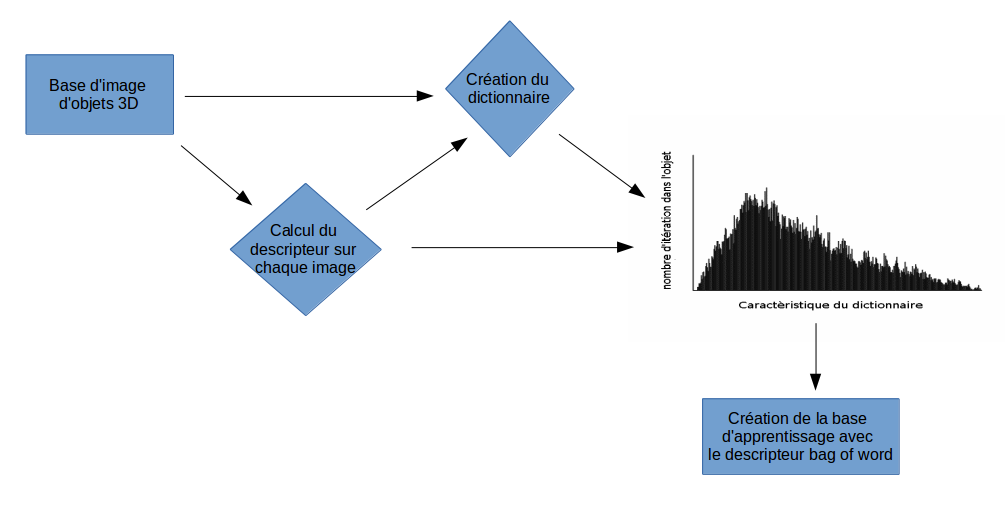
\includegraphics[height=8cm]{image/schemaBase.png}
    \caption{Schéma de la création de la base d'apprentissage}
  \end{center}
\end{figure}

%TODO parler des résultats de la reconnaissance

\subsection{Interface utilisateur}
L'interface utilisateur comprend deux fenêtres. La première comporte une vue avec le nuage de point récupérer à partir de la Kinect
et un ensemble d'option. Parmis ces options, nous avons la navigation dans le nuage de point et le choix de la technique de 
sélection. La première sélection est une simple sélection rectangulaire où l'ensemble des données à l'intérieur d'un rectangle formé
par deux points sont sélectionné. La second est une sorte de pinceau sélectionnant les données en dessous de la souris et celles dans 
un voisinage d'une taille variable. Lorsque l'utilisateur a sélectionné un objet et que l'application l'a reconnu, un nombre n de case 
avec des objets apparaît. Les objets dans ces cases sont les mêmes que l'objet sélectionné. Lorsque l'utilisateur clique sur l'une 
de ces cases, l'objets correspondant est ajouté dans la seconde fenêtre.
La second fenêtre contient l'environnement final dans lequel il y a déjà une piéce modèlisé avec des objets 3D. L'objet sélectionné est 
ajouté dans cette environnement.

\begin{figure}[!h]
  \begin{center}
    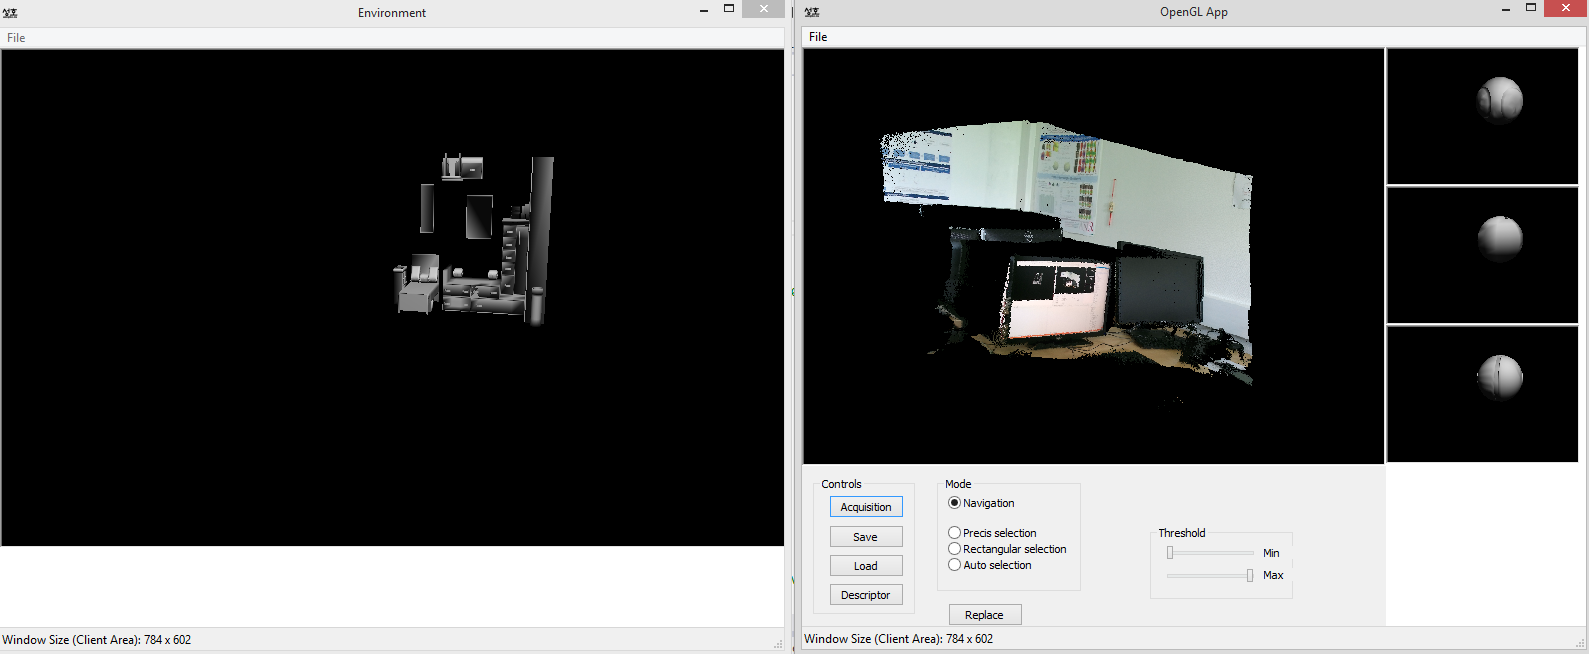
\includegraphics[height=7cm]{image/appliObjet.PNG}
    \caption{Interface de la seconde application}
  \end{center}
\end{figure}
